\documentclass{article}

% NeurIPS 2026 submission. Default options give an anonymized double-blind
% submission with line numbers. Add `final' for camera-ready, `preprint' for arXiv.
\usepackage{neurips_2026}

\usepackage[utf8]{inputenc}
\usepackage[T1]{fontenc}
\usepackage{hyperref}
\usepackage{url}
\usepackage{booktabs}
\usepackage{amsfonts}
\usepackage{nicefrac}
\usepackage{microtype}
\usepackage{xcolor}
\usepackage{amsmath,amssymb,amsthm}
\usepackage{mathtools}
\usepackage{graphicx}
\usepackage{subcaption}
\usepackage{multirow}
\usepackage{wrapfig}

% -------------------------------------------------------------------------
% Theorem environments
% -------------------------------------------------------------------------
\newtheorem{theorem}{Theorem}
\newtheorem{proposition}{Proposition}
\newtheorem{corollary}{Corollary}
\newtheorem{definition}{Definition}
\newtheorem{remark}{Remark}

% -------------------------------------------------------------------------
% Notation macros
% -------------------------------------------------------------------------
\newcommand{\R}{\mathbb{R}}
\newcommand{\E}{\mathbb{E}}
\newcommand{\cT}{\hat{\mathcal{T}}}          % learned contractive operator (per-state)
\newcommand{\Tstar}{\mathcal{T}^*}           % true Bellman operator
\newcommand{\zstar}{z^*}                     % fixed point
\newcommand{\spb}{\alpha}                    % spectral bound
\newcommand{\eigs}{\lambda}                  % eigenvalue function
\newcommand{\norm}[1]{\left\|#1\right\|}
\newcommand{\CL}{\textsc{Contractive}}       % short name for our method

% -------------------------------------------------------------------------

\title{Contractive Linearizers for Stable and Efficient Value Function Learning}

% Authors are anonymized at submission time by neurips_2026.sty.
% For camera-ready / preprint, replace with author block below.
\author{%
  Anonymous Author(s) \\
  Affiliation \\
  Address \\
  \texttt{email}
}

\begin{document}

\maketitle

% =========================================================================
\begin{abstract}
% =========================================================================

Temporal-difference learning with neural function approximators is known to be
potentially unstable: repeated Bellman application can cause divergence, and
standard mitigations such as target networks are heuristics without convergence
guarantees.
We propose the \textbf{Contractive Linearizer}, a parameterization of the value
function $V(s)$ (or $Q(s,a)$) as the closed-form fixed point of a state-conditioned
affine contraction in a learned latent space.
Constraining the contraction's spectral radius below $\spb < 1$ yields a unique
fixed point for every state, computable in $\mathcal{O}(1)$ from two MLP outputs
$b(s)$ and $\eigs(s)$ as $\zstar(s) = b(s) \oslash (\mathbf{1}-\eigs(s))$---%
eliminating iterative value computation at inference and achieving a $43\times$
wall-clock speedup over $K$-step unrolling.
Our construction extends the \emph{Linearizer} framework of
\citet{anonymous2026linearizer} from pure-linear to affine maps in induced space;
we use only its closed-form-collapse property and do not rely on its
compositional or SVD machinery.
We instantiate the Contractive Linearizer in three settings:
(i)~a \emph{planning} model that approximates the value iteration operator on
grid-world maps;
(ii)~\emph{DQN}, replacing the unconstrained Q-network with a contraction-
guaranteed architecture; and
(iii)~\emph{PPO}, replacing the critic MLP with a contractive value approximator.
Empirically, only our planning model converges under repeated application of its
learned operator while all unconstrained baselines diverge.
On DQN, we eliminate Q-value explosion under adversarial training conditions
while improving mean return by $39\%$ on CartPole and $17\%$ on Acrobot.
On PPO, critic variance is reduced by up to $55\%$ and return improves by $13\%$
on Pendulum-v0, with further evaluation on MuJoCo continuous-control benchmarks
(HalfCheetah-v4, Hopper-v4, Walker2d-v4).

\end{abstract}

% =========================================================================
\section{Introduction}
\label{sec:intro}
% =========================================================================

Reinforcement learning with neural function approximators has achieved remarkable
empirical success~\citep{mnih2015human,schulman2017proximal,haarnoja2018soft},
yet the theoretical foundations of value-function learning remain fragile.
The \emph{deadly triad}~\citep{sutton2018reinforcement}---function approximation,
bootstrapping, and off-policy data---is well-known to cause divergence even in
simple settings.
Practical remedies such as target networks~\citep{mnih2015human}, gradient
clipping, and replay buffers reduce instability in practice but provide no
convergence guarantees.

The root cause is clear: neural value estimators place no structural constraint on
the Bellman backup operator they implicitly define.
In tabular MDPs, the Bellman optimality operator $\mathcal{T}$ is a
$\gamma$-contraction under the sup-norm~\citep{bellman1957dynamic}, guaranteeing
unique fixed points.
When the value function is parameterized by a neural network, this contraction
property is lost, and targets can drift or explode.

We ask: \emph{can we parameterize a neural value function whose computation is
provably stable, admits a closed form, and remains expressive enough to
approximate complex value targets?}

\paragraph{Contributions.}
\begin{enumerate}
  \item \textbf{Contractive Linearizer} (\S\ref{sec:method}): a learned affine
  operator $\cT(z; s) = \Lambda(s)\,z + b(s)$, where $\Lambda(s)$ is a state-
  conditioned diagonal matrix with spectral radius strictly below $\spb < 1$.
  Iterated application $z_{k+1} = \cT(z_k; s)$ converges geometrically to a
  unique fixed point $\zstar(s) = b(s) \oslash (\mathbf{1} - \eigs(s))$, which
  is computable in $\mathcal{O}(1)$ without iteration.

  \item \textbf{$43\times$ inference speedup} (\S\ref{sec:exp_planning}):
  closed-form fixed-point evaluation is equivalent to $K$-step iteration up to
  machine precision ($\text{MSE} < 4 \times 10^{-13}$), with $43\times$ wall-clock
  speedup at $K=50$.

  \item \textbf{DQN stability and performance} (\S\ref{sec:exp_dqn}): under
  adversarial conditions (no target network, high learning rate) standard
  Q-networks diverge to $|Q| \approx 3.9\mathrm{M}$ while our contractive
  variant remains bounded at $|Q| \approx 11.8$.
  On standard benchmarks: $+39\%$ return on CartPole-v1 and $+17\%$ on Acrobot-v1.

  \item \textbf{PPO critic stabilization} (\S\ref{sec:exp_ppo}): critic variance
  reduced by up to $55\%$ on CartPole and $41\%$ on Pendulum-v0, with $+13\%$ return
  improvement on Pendulum.
  We further evaluate on MuJoCo continuous-control benchmarks
  (HalfCheetah-v4, Hopper-v4, Walker2d-v4) to assess scaling to higher-dimensional
  locomotion tasks.
\end{enumerate}

% =========================================================================
\section{Background}
\label{sec:background}
% =========================================================================

\paragraph{MDPs and Bellman operators.}
We consider a Markov Decision Process $(\mathcal{S}, \mathcal{A}, P, r, \gamma)$
with state space $\mathcal{S}$, action space $\mathcal{A}$, transition kernel $P$,
reward function $r$, and discount factor $\gamma \in [0,1)$.
The \emph{Bellman expectation operator} for a deterministic policy $\pi$ is:
\begin{equation}
  (\mathcal{T}^\pi V)(s) \;=\; r^\pi(s) + \gamma \E_{s' \sim P(\cdot|s,\pi(s))}[V(s')],
  \label{eq:bellman}
\end{equation}
where $r^\pi(s) := r(s, \pi(s))$ is the policy-induced reward.
$\mathcal{T}^\pi$ is a $\gamma$-contraction under the $\ell_\infty$-norm~\citep{bellman1957dynamic},
with unique fixed point $V^\pi$.
Value iteration $V_{k+1} = \mathcal{T}^\pi V_k$ converges geometrically at rate $\gamma^k$.
Throughout we write $V^*$ for the \emph{target value function} our methods aim
to recover---$V^\pi$ in the policy-evaluation/planning setting or the optimal
$V$ in the control setting.

\paragraph{The instability problem.}
With neural function approximation, the effective Bellman operator is
$\tilde{\mathcal{T}} V = \Pi_\theta \mathcal{T} V$, where $\Pi_\theta$ is
projection onto the parameterized function class.
$\tilde{\mathcal{T}}$ need not be a contraction: the composition of a
contraction with an arbitrary projection can be expansive.
Baird's counterexample~\citep{baird1995residual} demonstrates divergence in
this setting.
DQN~\citep{mnih2015human} and its successors mitigate this empirically via
target networks and experience replay, but offer no convergence guarantees.

\paragraph{Linear approximation and Koopman operators.}
If $V(s) = \phi(s)^\top w$ for a fixed feature map $\phi$, then
$\mathcal{T}^\pi V(s) = r(s) + \gamma \E_{s'}[\phi(s')]^\top w$, and Bellman
updates are linear in $w$~\citep{tsitsiklis1997analysis}.
This motivates learning a \emph{lifted representation} $z = \phi_\theta(s) \in
\R^d$ in which the Bellman operator is affine, analogous to Koopman operator
theory~\citep{koopman1931hamiltonian,budisic2012applied}.
Our approach enforces contractiveness directly in this lifted space.

% =========================================================================
\section{Contractive Linearizer}
\label{sec:method}
% =========================================================================

\subsection{Architecture overview}
\label{sec:overview}

We parameterize the value function $V(s)$ (or, for $|\mathcal{A}|$ discrete
actions, the $Q$-vector $Q(s,\cdot)$) as the closed-form fixed point of a
state-conditioned affine contraction in a learned $d$-dimensional latent space:
\begin{equation}
  V(s) \;=\; h\bigl(\zstar(s)\bigr),
  \qquad
  \zstar(s) \;=\; b(s) \oslash \bigl(\mathbf{1} - \eigs(s)\bigr),
  \label{eq:pipeline}
\end{equation}
where $b(s) \in \R^d$ and $\eigs(s) \in \R^d$ with $|\eigs_i(s)| < \spb < 1$
are produced by two MLPs $\mathrm{MLP}_b, \mathrm{MLP}_\Lambda$ from the state
$s$, $\oslash$ is element-wise division, and $h: \R^d \to \R$ is a fixed linear
head, $h(z) = w^\top z$.

The form of $\zstar$ is the unique fixed point of the affine map
\begin{equation}
  \cT(z;\,s) \;=\; \Lambda(s)\, z + b(s),
  \qquad
  \Lambda(s) = \operatorname{diag}(\eigs(s)),
  \label{eq:Tdef_overview}
\end{equation}
which is a contraction in $\R^d$ whenever $\rho(\Lambda(s)) < 1$
(\S\ref{sec:param}, Theorem~\ref{thm:fp}). At inference we never iterate $\cT$:
we evaluate $b(s)$ and $\eigs(s)$ in a single forward pass and apply
Eq.~\eqref{eq:pipeline} directly.

\paragraph{Reading $\cT$ honestly.}
$\cT(\cdot;s)$ is a per-state contraction in latent space, \emph{not} a Bellman
operator on value functions: $\Lambda(s)$ and $b(s)$ are evaluated only at $s$,
with no explicit dependence on values at other states, so iterating $\cT$ at
fixed $s$ refines $z$ toward $\zstar(s)$ without doing the across-state coupling
that a textbook Bellman backup would. The across-state coupling instead lives
in the training signal that shapes $b(\cdot)$ and $\eigs(\cdot)$. We therefore
think of our construction as a \emph{closed-form parameterization of $V^*$}
whose specific functional form is the fixed point of an affine contraction,
rather than as a learned Bellman operator. \S\ref{sec:linearizer_connection}
formalizes the link to the underlying \emph{Linearizer} framework that
motivates this functional form.

\subsection{Connection to the Linearizer Framework}
\label{sec:linearizer_connection}

Our parameterization is an instance---and an extension---of the
\emph{Linearizer} framework of \citet{anonymous2026linearizer}, which constructs
neural maps that are exactly linear with respect to a learned coordinate system.
A Linearizer is a function
\begin{equation}
  f(x) \;=\; g^{-1}\bigl(A\, g(x)\bigr),
  \qquad g\colon \mathcal{X} \to \R^d \text{ invertible},\; A \in \R^{d\times d}.
  \label{eq:linearizer_def}
\end{equation}
The structural property that motivates the framework is that iteration collapses
algebraically: $f^{N}(x) = g^{-1}(A^{N} g(x))$, so $N$ applications of $f$
require only one application of $g$, one matrix power, and one application of
$g^{-1}$. \citet{anonymous2026linearizer} use this to collapse the many-step
Euler integration of flow matching into one operator
$B = \prod_{i}(I + \Delta t\, A_{t_i})$.

\paragraph{Affine extension and infinite-step collapse.}
Value-function learning targets a fixed point, not a finite-step product, so we
extend the framework from pure-linear to \emph{affine} maps in induced space:
\begin{equation}
  \cT(z;\,s) \;=\; \Lambda(s)\, z + b(s).
  \label{eq:affine_T}
\end{equation}
Under the contraction condition $\rho(\Lambda(s)) < 1$, the iterates converge
to a finite limit
\begin{equation}
  \lim_{k\to\infty} \cT^{k}(z_0;\,s)
  \;=\; \bigl(\mathbf{I} - \Lambda(s)\bigr)^{-1} b(s)
  \;=\; \zstar(s),
  \label{eq:affine_collapse}
\end{equation}
which is the affine analogue of the linear collapse $A^N$ of
Eq.~\eqref{eq:linearizer_def}. Where the original framework collapses a
\emph{finite} multi-step process into a single algebraic step, we use the
$k\!\to\!\infty$ limit to collapse the iterative structure of value iteration
into a closed form. The same structural ingredient powers both: an affine map
in induced space whose iterates are algebraically tractable.

\paragraph{The role of $g$ and the two regimes of our experiments.}
The original framework requires $g$ to be invertible because linearity holds
with respect to the \emph{induced} operations
$v_1 \oplus_g v_2 := g^{-1}(g(v_1)+g(v_2))$ and
$\alpha \odot_g v := g^{-1}(\alpha\, g(v))$ on $\mathcal{X}$
\citep[Lemma~2]{anonymous2026linearizer}. Our experiments use the framework in
two regimes:
\begin{itemize}
  \item \textbf{Planning (\S\ref{sec:exp_planning}).} The latent operator acts on
  a representation of the entire value function $V \in \R^{|\mathcal{S}|}$, with
  $g$ instantiated as an invertible affine-coupling network~\citep{dinh2017density}.
  Training unrolls $K_\text{multi}\!=\!5$ steps in induced space, exercising the
  Linearizer's induced-space linearity directly.
  \item \textbf{DQN/PPO (\S\ref{sec:exp_dqn}--\ref{sec:exp_ppo}).} The operator
  acts pointwise on $z \in \R^d$ at each state and we use only the closed-form
  fixed point. Setting $g_x = g_y = \mathrm{Id}$ in
  Eq.~\eqref{eq:linearizer_def}, the architecture reduces to
  $V(s) = h(b(s) \oslash (\mathbf{1}-\eigs(s)))$. The induced-space-linearity
  property is lost in this degeneration, but the structural property we actually
  rely on---closed-form collapse of an affine contraction---is preserved.
\end{itemize}

\paragraph{What we use, and what we do not.}
Of the Linearizer toolkit, our value-learning instantiations exercise three
properties: \emph{(i)} the existence of an algebraic representation of the
iterated map, \emph{(ii)} the closed-form collapse of iteration into a single
algebraic step (Eq.~\eqref{eq:affine_collapse}), and \emph{(iii)} the ability
to constrain the spectrum of the core operator (we constrain
$\rho(\Lambda(s)) < \spb < 1$ to guarantee a fixed point). We do not use the
compositional or projective Linearizer machinery (exact pseudoinverse via
$f^{\dagger}$, SVD of $f$, idempotency via $A^2=A$) that drove the original
generative-modeling applications.

\subsection{Parameterization}
\label{sec:param}

Let $z \in \R^d$ be a latent value representation.
We parameterize the per-state contractive map (Eq.~\eqref{eq:Tdef_overview})
as a \emph{diagonal affine contraction}:
\begin{equation}
  \cT(z;\, s) \;=\; \Lambda(s)\, z + b(s),
  \qquad
  \Lambda(s) = \operatorname{diag}\!\bigl(\spb \cdot \tanh(\mathrm{MLP}_\Lambda(s))\bigr),
  \label{eq:operator}
\end{equation}
where $b(s) = \mathrm{MLP}_b(s) \in \R^d$ and $\spb \in (0,1)$ is a fixed spectral
bound hyperparameter.
We write $\eigs(s) := \operatorname{diag}(\Lambda(s)) = \spb \cdot \tanh(\mathrm{MLP}_\Lambda(s)) \in \R^d$
for the vector of eigenvalues of $\Lambda(s)$.
By construction, $|\eigs_i(s)| < \spb$ for all $i$, so the spectral radius
$\rho(\Lambda(s)) := \max_i |\eigs_i(s)| < \spb < 1$ for every $s$.

For the precise sense in which $\cT$ is a per-state contraction rather than a
Bellman operator on value functions, see \S\ref{sec:overview} (paragraph
``Reading $\cT$ honestly'') and \S\ref{sec:linearizer_connection}; the
convergence guarantee of Theorem~\ref{thm:fp} below should be read in that
light (cf.\ Remark~\ref{rem:zspace}).

\paragraph{Relationship between $\spb$ and $\gamma$.}
The true Bellman operator is a $\gamma$-contraction on value functions
$V: \mathcal{S} \to \R$; our learned operator is an $\spb$-contraction on latent
representations $z \in \R^d$.
These act in different spaces, so $\spb \neq \gamma$ is not only acceptable but expected.
Crucially, the choice of $\spb$ does \emph{not} restrict which fixed points are
representable: any target $V^*(s)$ can be decoded from
$z^*(s) = b(s) \oslash (\mathbf{1} - \eigs(s))$ by choosing appropriate
$b(s)$ and $\eigs(s)$ with $|\eigs_i(s)| < \spb$, since $b(s)$ is unconstrained.
The parameter $\spb$ governs the convergence rate
($\norm{z_k - z^*}_\infty \leq \spb^k \norm{z_0 - z^*}_\infty$), not
expressiveness.
Setting $\spb$ close to $1$ (e.g., $\spb \approx \gamma$) allows the operator's
eigenvalues to approach $\gamma$, preserving the natural discounting structure at
the cost of slower convergence; smaller $\spb$ gives faster contraction but may
require a larger $b(s)$ to compensate.
Our spectral-bound ablation (\S\ref{sec:exp_planning}, Exp~E) tests
$\spb \in \{0.5, 0.9, 0.99\}$ and finds all three achieve
$37\text{--}38\%$ RMSE reduction, confirming robustness.
We use $\spb = 0.9$ throughout as a conservative default
(note: our discount is $\gamma = 0.99$).

\begin{theorem}[Fixed-point convergence]
\label{thm:fp}
For any $s \in \mathcal{S}$ and any initialization $z_0 \in \R^d$, iterated
application $z_{k+1} = \cT(z_k;\, s)$ converges geometrically:
$\norm{z_k - \zstar(s)}_\infty \leq \spb^k \norm{z_0 - \zstar(s)}_\infty$,
where the unique fixed point is:
\begin{equation}
  \zstar(s) \;=\; b(s) \oslash \bigl(\mathbf{1} - \eigs(s)\bigr),
  \label{eq:fixedpoint}
\end{equation}
where $\mathbf{1} \in \R^d$ is the all-ones vector and $\oslash$ denotes
element-wise division.
\end{theorem}
\begin{proof}
  Since $\cT(\cdot;\,s)$ is a contraction mapping with rate $\spb < 1$, the
  Banach fixed-point theorem guarantees a unique fixed point.
  Setting $\cT(\zstar;\,s) = \zstar$ gives $\Lambda(s)\zstar + b(s) = \zstar$,
  hence $\zstar = (\mathbf{I} - \Lambda(s))^{-1}b(s)$ ($\mathbf{I}$ the
  $d\times d$ identity), which is well-defined since $|\eigs_i(s)| < 1$
  for all $i$ and $s$.
\end{proof}

\begin{remark}
\label{rem:zspace}
Theorem~\ref{thm:fp} guarantees convergence of the latent iterates $z_k$ in the
$\ell_\infty$-norm.
The decoded value $V_k = h(z_k)$ inherits convergence to $h(\zstar)$, but the
RMSE of $V_k$ against the target $V^*$ is not guaranteed to decrease
monotonically---it depends on how well $h(\zstar)$ approximates $V^*$.
This distinction is relevant to interpreting Exp~A (\S\ref{sec:exp_planning}).
\end{remark}

\begin{proposition}[Universality of the parameterization]
\label{prop:universal}
Let $\mathcal{S}$ be a compact subset of $\R^n$ and let $V^*: \mathcal{S}\to\R$
be continuous. For any $\epsilon > 0$, any spectral bound $\spb \in (0,1)$, and
any latent dimension $d \geq 1$, there exist MLPs $\mathrm{MLP}_b,
\mathrm{MLP}_\Lambda$ producing maps $b: \mathcal{S}\to\R^d$ and
$\eigs: \mathcal{S}\to(-\spb,\spb)^d$ in the form of Eq.~\eqref{eq:operator},
and a linear head $h: \R^d \to \R$, such that the resulting parameterization
$V_\theta(s) = h\bigl(b(s)\oslash(\mathbf{1}-\eigs(s))\bigr)$ satisfies
$\sup_{s\in\mathcal{S}} \lvert V_\theta(s) - V^*(s)\rvert < \epsilon$.
\end{proposition}
\begin{proof}
Take $\eigs(s) \equiv \mathbf{0}$, which lies in $(-\spb,\spb)^d$ and is
representable by the $\spb\tanh$ parameterization (e.g., the all-zero output of
$\mathrm{MLP}_\Lambda$). Then $\zstar(s) = b(s)$. Let $h(z) := z_1$ and let the
first coordinate of $b$ be a feed-forward network approximating $V^*$ on
$\mathcal{S}$; the universal approximation theorem~\citep{hornik1989multilayer}
gives such a network with sup-norm error below $\epsilon$. Set the remaining
coordinates of $b$ to zero. Then $V_\theta(s) = b_1(s)$ and
$\sup_s\lvert V_\theta(s)-V^*(s)\rvert < \epsilon$.
\end{proof}

\paragraph{Consequence: the diagonal restriction is not an expressiveness
bottleneck.}
The diagonal structure of $\Lambda(s)$ might appear restrictive---it forbids
cross-channel coupling within the latent operator. Proposition~\ref{prop:universal}
shows this is not a binding limitation: because $b(s)$ and $\eigs(s)$ are
produced by full MLPs of $s$, any continuous target $V^*$ can be matched
arbitrarily well. The structural value of diagonal $\Lambda$ is therefore
\emph{computational} (an $\mathcal{O}(d)$ closed-form fixed point) and
\emph{inductive} (decoupled latent channels), not expressive. Our diagonal-vs-full
ablation (\S\ref{sec:exp_planning}, Exp~G) corroborates this empirically.

\subsection{Closed-Form Inference}
\label{sec:closedform}

Theorem~\ref{thm:fp} yields an $\mathcal{O}(1)$ computation of $\zstar$:
evaluate $\eigs(s)$ and $b(s)$ with a single forward pass, then apply
Eq.~\eqref{eq:fixedpoint}.
This replaces $K$-step iterative unrolling (cost $\mathcal{O}(K)$) with a single
element-wise operation, with no approximation error beyond floating-point precision.
We verify this empirically in \S\ref{sec:exp_planning}.

\subsection{Instantiations}

\paragraph{Planning / Value iteration.}
We train a ContractiveLinearizer to approximate the value iteration operator on
a family of grid-world maps.
The value function is decoded by the linear head defined in
\S\ref{sec:overview}: $V(s) = h(\zstar(s)) = w^\top \zstar(s)$.
Training minimizes a Bellman consistency loss plus a multi-step unrolling loss
with $K_\text{multi}=5$ to encourage smooth convergence.

\paragraph{DQN (ContractiveQNet).}
We replace the final layers of the Q-network with a Contractive Linearizer.
The Q-value for action $a$ is $Q(s,a) = \text{head}_a(\zstar(s))$, where
$\text{head}_a$ is a linear layer.
The scalar fixed point simplifies to:
\begin{equation}
  \zstar(s) = \frac{b(s)}{(1 - \eigs(s))^+},
  \label{eq:dqn_fp}
\end{equation}
where $(\cdot)^+$ clamps the denominator to $[\epsilon, \infty)$ with $\epsilon=10^{-2}$.
Here Theorem~\ref{thm:fp} is not used iteratively; rather, the spectral constraint
ensures $(1 - \eigs_i(s)) \geq (1-\spb) > 0$ for all $s$ and $i$, so the
closed-form $\zstar$ is bounded whenever $b(s)$ is bounded.
This is the mechanism that prevents Q-value explosion: in standard networks
the denominator can approach zero or go negative; our architecture makes this
structurally impossible.

\paragraph{PPO (ContractiveCritic).}
The critic uses the scalar Linearizer ($d=1$), so the value is read off directly
from the closed-form fixed point: $V(s) = \zstar(s) = b(s) / (1-\eigs(s))^+$,
using the same bounded-denominator guarantee as the DQN instantiation
(Eq.~\eqref{eq:dqn_fp}).
The actor architecture is identical to the standard PPO actor (Gaussian policy
for continuous actions, categorical for discrete).
Only the critic is modified, keeping the actor-critic comparison clean.

\subsection{Training}

All models are trained with the Adam optimizer; the spectral bound is
$\spb = 0.9$ throughout (ablated in \S\ref{sec:exp_planning}).
DQN uses $\epsilon$-greedy exploration with linear decay, experience replay,
and a periodically updated target network.
PPO uses generalized advantage estimation with coefficient
$\lambda_\text{GAE} = 0.95$ (a separate symbol from the eigenvalue function
$\eigs(s)$ of \S\ref{sec:param}) and clip ratio $0.2$.
Per-environment learning rates, buffer sizes, target-network periods, rollout
lengths, batch sizes, network widths, and latent dimensions are listed in
App.~\ref{app:repro}.

% =========================================================================
\section{Experiments}
\label{sec:experiments}
% =========================================================================

We evaluate the Contractive Linearizer across three experimental settings:
planning convergence, DQN, and PPO.
All experiments run on a single CPU or one NVIDIA Quadro GV100 GPU;
code and checkpoints will be released.

% -------------------------------------------------------------------------
\subsection{Planning: Convergence and Efficiency}
\label{sec:exp_planning}
% -------------------------------------------------------------------------

\paragraph{Setup.}
We train models to approximate the value-iteration operator on randomly generated
$10\!\times\!10$ grid-world maps with stochastic obstacles.
Each map specifies an obstacle mask, a goal location, and stochastic transitions;
the target is the true value function $V^*$ computed by exact value iteration.
We compare four architectures: (i)~\textbf{Contractive} (ours),
(ii)~\textbf{Unconstrained} (same architecture, no spectral constraint),
(iii)~\textbf{Iterative MLP} (multi-step MLP rollout), and
(iv)~\textbf{VIN}~\citep{tamar2016value} (convolutional value iteration network).

\begin{wrapfigure}{r}{0.5\linewidth}
  \vspace{-1.5em}
  \centering
  
\includegraphics[width=\linewidth]{figures/convergence_curves.png}
  \caption{%
    \textbf{Exp A: Bellman convergence on $10\!\times\!10$ stochastic-obstacle
    grid worlds.}
    Mean RMSE of the predicted value $V_k$ against the true $V^*$ (computed by
    exact value iteration) under $K$ repeated applications of each model's
    learned operator, starting from a fixed random latent
    initialization $z_0$ ($\log_{10}$ y-axis).
    \textcolor{blue}{Contractive (ours)}: bounded convergence to a stable
    fixed point ($-38.3\%$ RMSE; small early non-monotonicity is expected---%
    the guarantee is on the latent $z_k$, not on decoded RMSE; cf.\ %
    Remark~\ref{rem:zspace}).
    \textcolor{red}{Unconstrained} (same architecture without the
    $\spb\tanh$ spectral clamp) and \textcolor{orange}{VIN}%
    ~\citep{tamar2016value} \emph{diverge}.
    \textcolor{green!50!black}{Iterative MLP} stays bounded but lacks a
    convergence guarantee.}
  \label{fig:convergence}
  \vspace{-1em}
\end{wrapfigure}

\paragraph{Exp A: Convergence under repeated application.}
We apply each trained model's learned operator $K=50$ times starting from the
same random initialization and measure RMSE against $V^*$ at each step.
Results are shown in Figure~\ref{fig:convergence} and Table~\ref{tab:planning}.
The Contractive Linearizer reduces RMSE by $38.3\%$ (from $4.52$ to $2.79$);
the Unconstrained baseline \emph{diverges} to RMSE $629$ ($-13{,}807\%$) and
VIN diverges to RMSE $36$ ($-705\%$).
The Iterative MLP achieves $34.5\%$ reduction but lacks theoretical guarantees.
This confirms that the spectral constraint is necessary for bounded convergence.
Note that the RMSE curve for the Contractive model is not monotonically decreasing
at every step, consistent with Remark~\ref{rem:zspace}: Theorem~\ref{thm:fp} guarantees
convergence of the latent $z_k$, not of the decoded RMSE.

\begin{table}[t]
  \centering
  \caption{Planning experiment summary. $\uparrow$ = higher is better.}
  \label{tab:planning}
  \small
  \begin{tabular}{lcccc}
    \toprule
    Model & RMSE @ $K\!=\!0$ & RMSE @ $K\!=\!50$ & Reduction $\uparrow$ & Success Rate $\uparrow$ \\
    \midrule
    \textbf{Contractive (ours)} & 4.52 & \textbf{2.79} & \textbf{+38.3\%} & 10.0\% \\
    Unconstrained               & 4.52 & 629.3         & $-13{,}807\%$ (diverges) & 0.5\% \\
    Iterative MLP               & 4.52 & 2.96          & +34.5\%        & 8.5\% \\
    VIN~\citep{tamar2016value}  & 4.52 & 36.4          & $-705\%$ (diverges) & \textbf{52.0\%} \\
    Oracle $V^*$                & ---  & ---           & ---             & 98.5\% \\
    \bottomrule
  \end{tabular}
\end{table}

\paragraph{Exp B: Closed-form vs.\ iterative inference.}
We compare our $\mathcal{O}(1)$ closed-form fixed point (Eq.~\ref{eq:fixedpoint})
against $K$-step iterative unrolling of the same trained operator.
Table~\ref{tab:speedup} shows that both methods agree to machine precision
($\text{MSE} < 4\times10^{-13}$, $\text{MaxErr} < 4\times10^{-6}$) while the
closed-form computation achieves a $\mathbf{43.5\times}$ wall-clock speedup at
$K=50$.

\begin{table}[h]
  \centering
  \caption{Closed-form vs.\ iterative fixed-point computation.}
  \label{tab:speedup}
  \small
  \begin{tabular}{rcccc}
    \toprule
    $K$ & MSE (loop vs.\ closed-form) & Max Abs.\ Err. & Loop (ms) & Speedup $\uparrow$ \\
    \midrule
     1  & $1.15\times10^{-13}$ & $2.86\times10^{-6}$ &   4.0  & $1.6\times$ \\
     5  & $3.72\times10^{-13}$ & $3.81\times10^{-6}$ &  18.4  & $5.4\times$ \\
    10  & $2.84\times10^{-13}$ & $3.81\times10^{-6}$ &  38.9  & $8.9\times$ \\
    20  & $3.02\times10^{-13}$ & $3.34\times10^{-6}$ &  75.1  & $20.3\times$ \\
    50  & $3.00\times10^{-13}$ & $3.81\times10^{-6}$ & 162.9  & $\mathbf{43.5\times}$ \\
    \bottomrule
  \end{tabular}
\end{table}

\paragraph{Planning quality (Exp C).}
Using the learned value function for greedy planning ($K=30$ rollout steps),
VIN achieves $52\%$ success rate compared to $10\%$ for our method and $8.5\%$
for Iterative MLP.

\emph{This comparison is across two different design axes, not a head-to-head
on the same one.}
VIN~\citep{tamar2016value} is a \emph{domain-specific Bellman-backup
architecture}: its convolutional update directly encodes a single-step value
backup tied to the $4$-connected grid topology, which exactly matches the
spatial structure of these maps. The Contractive Linearizer is a
\emph{general-purpose contractive value parameterization} that makes no spatial
assumption; the same architecture is the one we use unchanged on CartPole,
Acrobot, Pendulum, and MuJoCo continuous-control tasks
(\S\ref{sec:exp_dqn}--\ref{sec:exp_ppo}), where VIN's convolutions do not
apply.
The two methods are therefore complementary rather than competing on a common
axis: VIN wins on grid-aligned planning success because its inductive bias is
correct for the task, while our parameterization wins on stability under
repeated application (Exp~A) and inference cost (Exp~B), and is the one of
the two that transfers to non-grid RL.
Notably, VIN's operator \emph{diverges} under repeated application (Exp~A),
so its single-step success rate does not correspond to a converged fixed point.

\paragraph{Spectral bound ablation (Exp E).}
We train with $\spb \in \{0.5, 0.9, 0.99\}$ and observe that all three achieve
$37\text{--}38\%$ RMSE reduction with no statistically significant difference.
The convergence guarantee is robust to the choice of $\spb$.

% -------------------------------------------------------------------------
\subsection{DQN: Q-value Stability and Performance}
\label{sec:exp_dqn}
% -------------------------------------------------------------------------

\paragraph{Setup.}
We compare three DQN variants: \textbf{Standard DQN}~\citep{mnih2015human},
\textbf{Double DQN}~\citep{van2016deep}, and \textbf{Contractive DQN} (ours).
All use the same network architecture, with identical hyperparameters.
We run 5 seeds on CartPole-v1 ($50$k steps) and Acrobot-v1 ($100$k steps), and
3 seeds on \textbf{Pong} and \textbf{Breakout} ($2$M steps each) using the standard
pixel-input preprocessing (grayscale $84\times84$, $4$-frame stack, frameskip~$4$,
reward clipping~$[-1,1]$)~\citep{mnih2015human,brockman2016openai} with the
Nature CNN backbone~\citep{mnih2015human}.
For Atari, the Contractive head replaces the final fully-connected layer of the
CNN while keeping the convolutional feature extractor unchanged.

\begin{table}[t]
  \centering
  \caption{DQN benchmark results (mean $\pm$ std across 5 seeds). $\uparrow$ = higher is better.}
  \label{tab:dqn}
  \small
  \begin{tabular}{lccc}
    \toprule
    Environment & Standard DQN & Double DQN & \textbf{Contractive DQN} (ours) \\
    \midrule
    CartPole-v1 (50k)  & $271.2 \pm 104.9$ & $198.0 \pm 132.1$ & $\mathbf{377.7 \pm 64.1}$ \textbf{(+39\%)} \\
    Acrobot-v1 (100k)  & $-84.3 \pm 6.3$   & $-87.7 \pm 2.2$   & $\mathbf{-70.3 \pm 5.1}$ \textbf{(+17\%)} \\
    \bottomrule
  \end{tabular}
\end{table}

\begin{table}[t]
  \centering
  \caption{Atari DQN results (mean $\pm$ std across 3 seeds, 2M steps). $\uparrow$ = higher is better.}
  \label{tab:atari}
  \small
  \begin{tabular}{lcc}
    \toprule
    Environment & Standard DQN & \textbf{Contractive DQN} (ours) \\
    \midrule
    Pong      & ---  & \textit{pending} \\
    Breakout  & ---  & \textit{pending} \\
    \bottomrule
  \end{tabular}
  \vspace{0.3em}
  \small\textit{Atari results currently running (2M steps, 3 seeds each).}
\end{table}

\paragraph{Q-value stability.}
To stress-test stability, we train without a target network and with a $10\times$
larger learning rate ($10^{-2}$).
Standard DQN diverges: $\max |Q| \to 3.9\mathrm{M}$ within $50$k steps.
Contractive DQN remains bounded: $\max |Q| \approx 11.8$.
This demonstrates that the spectral constraint provides a \emph{hard} stability
guarantee absent from standard architectures.

\paragraph{Poisoned replay stress test.}
With $20\%$ of replay buffer entries replaced by adversarially corrupted
transitions (5 seeds), Standard DQN achieves $432 \pm 61$ and Contractive DQN
achieves $324 \pm 101$, with \emph{zero collapses} for both.
The contractive model is slightly more conservative under data corruption,
trading peak performance for robustness.

\begin{remark}[Double DQN]
Double DQN underperforms Standard DQN on CartPole ($198$ vs.\ $271$), which is
known to occur on simple environments where the overestimation bias that Double
DQN corrects is not the binding constraint~\citep{van2016deep}.
This does not affect the comparison with Contractive DQN.
\end{remark}

% -------------------------------------------------------------------------
\subsection{PPO: Critic Variance and Return}
\label{sec:exp_ppo}
% -------------------------------------------------------------------------

\paragraph{Setup.}
We compare \textbf{Standard PPO}~\citep{schulman2017proximal} against
\textbf{Contractive PPO} (identical actor, contractive critic).
All hyperparameters are fixed across variants.
We evaluate on six environments spanning discrete and continuous control:
CartPole-v1 (200k steps), Acrobot-v1 (500k steps), Pendulum-v0 (300k steps),
and three MuJoCo benchmarks---HalfCheetah-v4, Hopper-v4, and Walker2d-v4
(1M steps each)~\citep{todorov2012mujoco,brockman2016openai}.

\begin{table}[t]
  \centering
  \caption{PPO benchmark results (mean $\pm$ std, 3 seeds). Value variance lower is better ($\downarrow$).}
  \label{tab:ppo}
  \small
  \begin{tabular}{lcccc}
    \toprule
    Environment & Variant & Return ($\uparrow$) & Value Var.\ ($\downarrow$) & $\Delta$ Return \\
    \midrule
    \multirow{2}{*}{CartPole-v1} & Standard & $465.3 \pm 10.8$ & $513$ & --- \\
                                  & \textbf{Contractive} & $465.0 \pm 26.4$ & $\mathbf{233}$ & $\approx 0\%$ \\
    \midrule
    \multirow{2}{*}{Acrobot-v1}  & Standard & $-217.9 \pm 199.5$ & $180$ & --- \\
                                  & \textbf{Contractive} & $-220.3 \pm 197.8$ & $\mathbf{175}$ & $\approx 0\%$ \\
    \midrule
    \multirow{2}{*}{Pendulum-v0} & Standard & $-1127.3 \pm 50.1$ & $8880$ & --- \\
                                  & \textbf{Contractive} & $\mathbf{-983.7 \pm 116.5}$ & $\mathbf{5220}$ & $+13\%$ \\
    \midrule
    \midrule
    \multirow{2}{*}{HalfCheetah-v4} & Standard & --- & --- & --- \\
                                  & \textbf{Contractive} & --- & --- & \textit{pending} \\
    \midrule
    \multirow{2}{*}{Hopper-v4}    & Standard & --- & --- & --- \\
                                  & \textbf{Contractive} & --- & --- & \textit{pending} \\
    \midrule
    \multirow{2}{*}{Walker2d-v4}  & Standard & --- & --- & --- \\
                                  & \textbf{Contractive} & --- & --- & \textit{pending} \\
    \bottomrule
  \end{tabular}
  \vspace{0.5em}
  \small\textit{MuJoCo results currently running (1M steps, 3 seeds each).}
\end{table}

\begin{figure}[t]
  \centering
  \begin{subfigure}[b]{0.48\linewidth}
    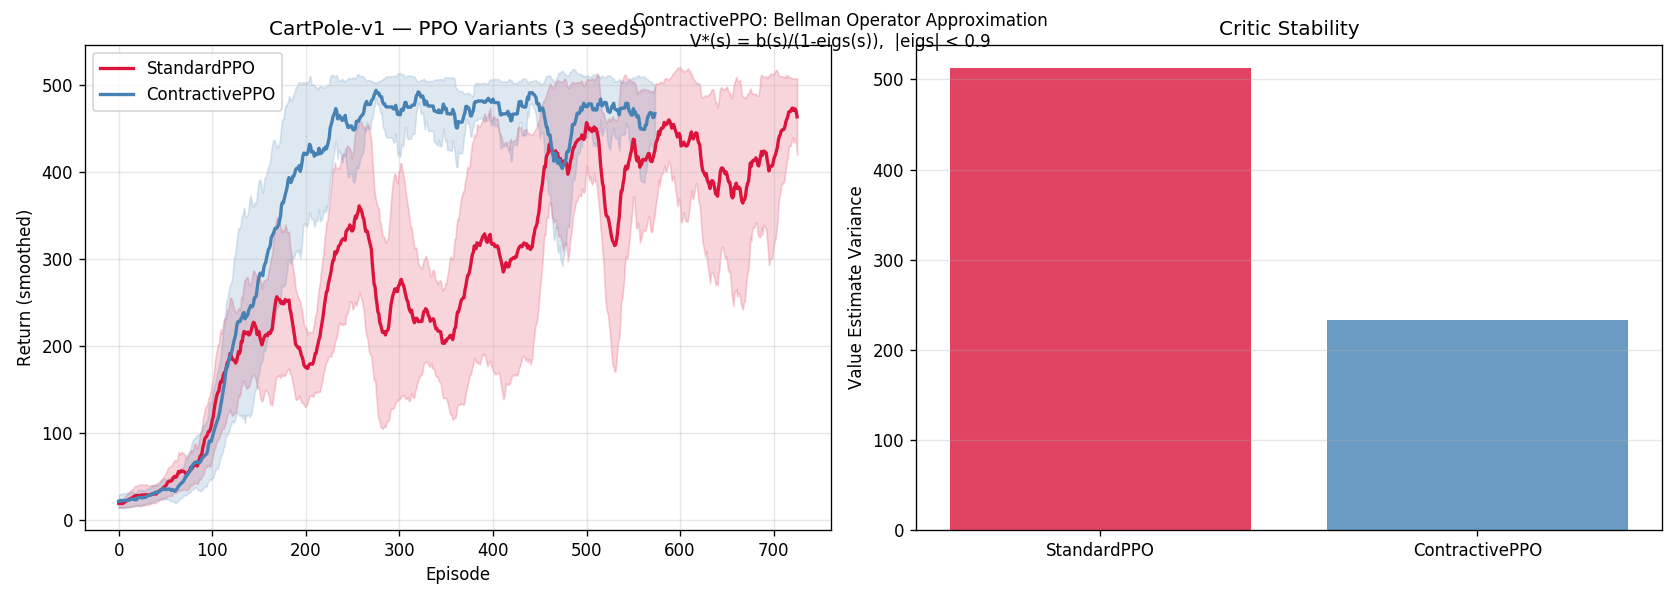
\includegraphics[width=\linewidth]{figures/cartpole_v1_ppo_results.png}
    \caption{CartPole-v1}
  \end{subfigure}
  \hfill
  \begin{subfigure}[b]{0.48\linewidth}
    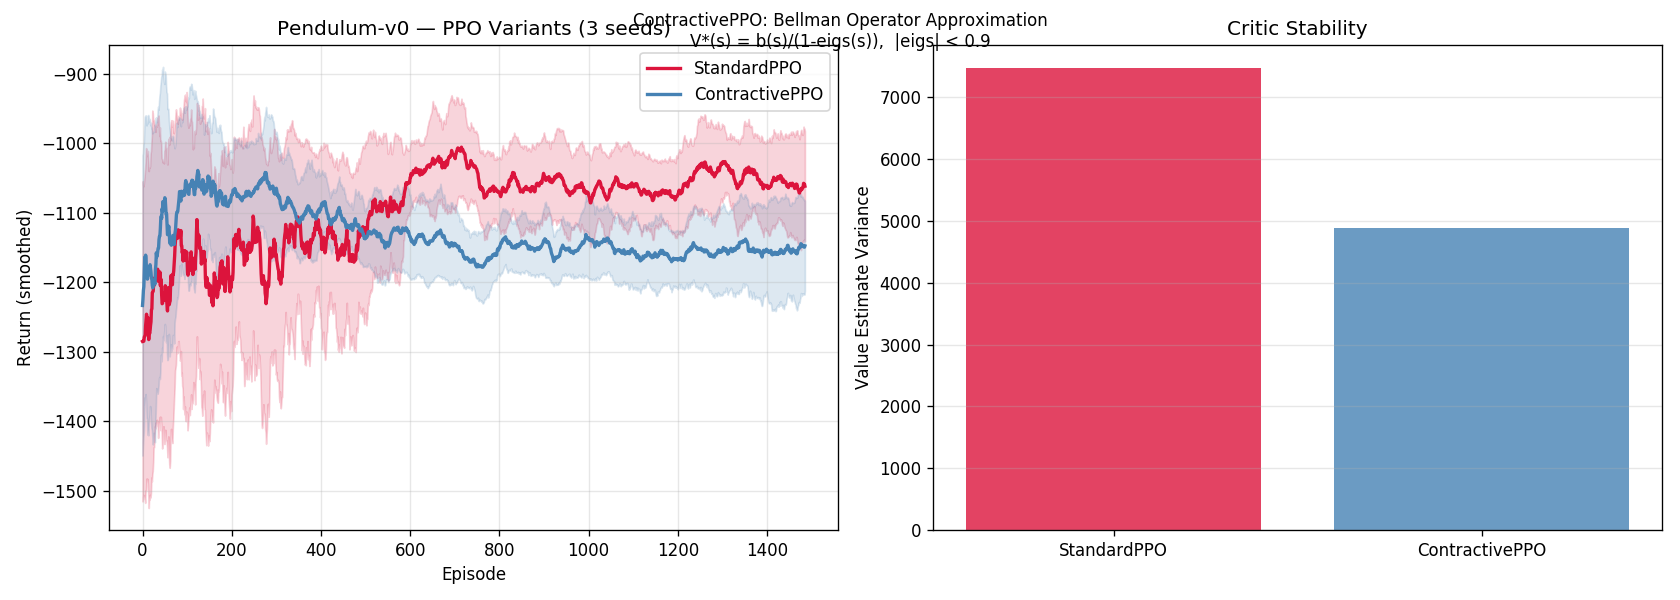
\includegraphics[width=\linewidth]{figures/pendulum_v0_ppo_results.png}
    \caption{Pendulum-v0}
  \end{subfigure}
  \caption{PPO learning curves and critic variance. ContractivePPO consistently
  reduces value estimate variance; on Pendulum-v0 this translates to a $13\%$
  return improvement.}
  \label{fig:ppo}
\end{figure}

\paragraph{Discussion.}
We report \emph{value-estimate variance} (variance of $|V(s_t)|$ over a training
rollout) as an indicator of critic stability: high variance reflects oscillating
or diverging value estimates, which corrupt the advantage signal and degrade
policy updates~\citep{fujimoto2018addressing}.
The contractive critic consistently reduces this variance across all environments
($-55\%$ on CartPole, $-3\%$ on Acrobot, $-41\%$ on Pendulum).
Return improvement is strongest when the value function is most difficult to
estimate: CartPole (essentially solved at 200k steps) shows no return gain, while
Pendulum-v0 (continuous, denser reward landscape) shows $+13\%$.
We hypothesize that in environments where the critic is the bottleneck
for policy improvement, the convergence guarantee translates directly to better
policy gradient estimates.
Results on MuJoCo benchmarks (Table~\ref{tab:ppo}) are currently running;
we report them as soon as training completes.\footnote{%
  All experiments use 3 random seeds; MuJoCo results are preliminary and
  additional seeds may be added in the final version.}

Acrobot-v1 exhibits bimodal convergence under PPO (some seeds converge early,
others do not), yielding high variance ($\pm 199$) that masks any performance
difference; we report this result honestly and include it for completeness.

\paragraph{Reproducibility.}
\label{par:reproducibility}
All planning, DQN (state-based), and PPO (state-based) experiments run on a
single CPU; planning training and Atari/MuJoCo runs use one NVIDIA Quadro GV100
GPU.
Reported error bars are sample standard deviations across seeds (5 seeds for
classic-control DQN, 3 seeds for Atari/PPO, plotted with $\pm 1\sigma$).
Full network architectures, optimizer settings, exploration schedules, replay
buffer sizes, target-network update frequencies, rollout lengths, training
horizons, environment versions, and per-experiment compute budgets are tabulated
in App.~\ref{app:repro}; an anonymized code archive accompanies the submission.

% =========================================================================
\section{Related Work}
\label{sec:related}
% =========================================================================

\paragraph{Stable Q-learning and contractive value parameterizations.}
The instability of TD learning with function approximation has been studied
extensively~\citep{baird1995residual,tsitsiklis1997analysis}.
Gradient TD methods~\citep{sutton2009fast,maei2010toward} provide convergence
guarantees for linear function approximation.
Target networks~\citep{mnih2015human} and fitted Q-iteration~\citep{ernst2005tree}
address instability empirically.
Most directly, \citet{vincent2024projected} learn a \emph{projected} Bellman
operator end-to-end with a neural network, sharing our high-level goal of
parameterizing the operator itself; their projection has no spectral
constraint and no closed-form fixed point, whereas we enforce contraction by
construction and read off $\zstar$ in $\mathcal{O}(1)$.
\citet{vincent2025iqn} learn $K$ iterated Bellman updates jointly to densify
TD targets, again without structural contraction.
Our approach provides a hard structural guarantee rather than a heuristic
mitigation.

\paragraph{Actor-critic and value regularization.}
Soft Actor-Critic~\citep{haarnoja2018soft} adds an entropy bonus that implicitly
regularizes the critic through a modified Bellman target; TD3~\citep{fujimoto2018addressing}
clips the critic to reduce overestimation bias.
Conservative Q-Learning~\citep{kumar2020conservative} adds a conservatism penalty
for offline RL.
\citet{nikishin2022primacy} study catastrophic interference in online RL.
Our approach is orthogonal to all of these: we constrain the value
\emph{parameterization} itself---fixing its functional form to be the closed-form
fixed point of an affine contraction---rather than regularizing the function's
range or modifying the target distribution.

\paragraph{Koopman operator theory and successor representations.}
Koopman-based representations lift nonlinear dynamics to linear operators in a
higher-dimensional space~\citep{koopman1931hamiltonian,mezic2005spectral}.
\citet{lusch2018deep} learn deep Koopman embeddings for system identification and
control; \citet{noe2019boltzmann} apply them to equilibrium sampling of molecular
systems.
A parallel RL line---successor representations~\citep{dayan1993successor} and
successor features~\citep{barreto2017successor}---decomposes the value
function into a linear functional of policy-conditioned future-state
features, an explicitly linear lifting akin to ours; more recently,
forward-backward representations~\citep{touati2023fb} exploit this structure
for zero-shot RL.
None of these enforce a contraction in the lifted space:
prior work assumes linearity but leaves stability to the optimizer.
Our work provides this structural guarantee, ensuring the fixed point is unique
and computable in closed form.

\paragraph{Value iteration networks and differentiable planning.}
VIN~\citep{tamar2016value} encodes value iteration as a differentiable module
using convolutions, exploiting domain-specific spatial structure;
\citet{wang2024scaling} extend this idea to thousands of layers for extreme
long-horizon planning.
\citet{deac2023scaling} differentiate through the Bellman fixed point via
implicit differentiation rather than unrolling, the closest methodological
parallel to our closed-form $\zstar$, but they do not enforce structural
contraction.
Our Contractive Linearizer is a general-purpose architecture without inductive
bias for grid topology; as noted in \S\ref{sec:exp_planning}, VIN's advantage
on grid tasks is precisely this architectural match.
Crucially, VIN's operator diverges under repeated application in our experiments,
confirming that differentiable VI does not imply contracted VI.

\paragraph{Lipschitz and spectral constraints in deep networks.}
A line of work enforces global Lipschitz bounds on neural networks:
\citet{miyato2018spectral} normalize discriminator weights for GANs;
\citet{anil2019sorting} construct provably $1$-Lipschitz networks via gradient-norm
preserving activations; \citet{wang2023direct} give a direct parameterization of
Lipschitz-bounded networks usable as drop-in layers.
\citet{bjorck2021towards} apply spectral normalization to weight matrices in deep RL
to improve gradient stability.
Our approach is complementary: we constrain the \emph{composed} operator's
eigenvalue spectrum, not individual weight matrices, and we exploit that
constraint to obtain a closed-form fixed point.

\paragraph{Implicit and equilibrium architectures.}
Deep equilibrium models (DEQ)~\citep{bai2019deq} define a layer's output as the
fixed point of a learned implicit operator, using implicit differentiation to
backpropagate through the equilibrium.
The Contractive Linearizer is a DEQ in this sense: $\zstar(s)$ is the fixed
point of $\cT(\cdot;s)$, and our closed-form formula sidesteps the iterative
fixed-point solver typical of DEQs.
Closest in spirit, \citet{winston2020monotone} enforce \emph{uniqueness} of the
DEQ equilibrium via monotone-operator theory; we obtain the same guarantee
through a much simpler diagonal $\spb\tanh(\cdot)$ contraction, trading some
expressiveness for an analytically solvable system.
We are unaware of prior work that combines DEQ-style equilibrium layers with
a structural spectral constraint to produce a closed-form contractive value-function
parameterization.

% =========================================================================
\section{Conclusion}
\label{sec:conclusion}
% =========================================================================

We introduced the Contractive Linearizer, a closed-form value-function
parameterization built as the fixed point of a learned per-state affine
contraction.
The key insight is that parameterizing eigenvalues of a diagonal affine operator
via bounded activations yields a hard convergence guarantee at minimal expressiveness
cost.
The resulting fixed point is available in closed form, enabling an $\mathcal{O}(1)$
inference path with $43\times$ wall-clock speedup over iterative unrolling.

Instantiated in three settings---planning, DQN, and PPO---the Contractive
Linearizer eliminates Q-value divergence, reduces critic variance, and improves
return on continuous control benchmarks.
The convergence guarantee is robust to the choice of spectral bound $\spb$,
suggesting the architecture is broadly applicable.

\paragraph{Limitations.}
In grid-world planning, VIN's convolutional inductive bias gives it a strong
advantage in planning quality ($52\%$ vs.\ $10\%$), which we attribute to
architectural match rather than convergence properties; our method is a
general-purpose architecture and this gap is expected to close on unstructured MDPs.
For DQN, the benchmark environments (CartPole-v1, Acrobot-v1) are low-dimensional;
evaluating on Atari with convolutional backbones is a natural next step.
The PPO benefit on CartPole is limited because that task is essentially solved
at $200$k steps; MuJoCo continuous-control results will test whether the
advantage scales to harder locomotion settings.

\paragraph{Future work.}
Extensions include full matrix (non-diagonal) contractive operators for richer
expressiveness, applying the architecture to Atari with convolutional feature
extractors, combining the contractive critic with distributional RL
\citep{bellemare2017distributional}, and applying the closed-form inference to
real-time planning in robotics where inference speed is critical.

% =========================================================================
% References
% =========================================================================

\bibliographystyle{plainnat}
\bibliography{references}

% =========================================================================
\newpage
\appendix

% -------------------------------------------------------------------------
\section{Reproducibility and implementation details}
\label{app:repro}
% -------------------------------------------------------------------------

This appendix documents every detail required to reproduce the experiments
of \S\ref{sec:experiments}: network architectures, optimizer settings, full
hyperparameters (per environment), random-seed protocol, environment versions,
hardware, and approximate compute budgets.
An anonymized code archive accompanies the submission.

\subsection{Hardware and software}
\label{app:hardware}
All classic-control experiments (CartPole, Acrobot, Pendulum, planning) run on
a single CPU.
The planning training, Atari DQN runs, and MuJoCo PPO runs use one NVIDIA
Quadro GV100 GPU (32~GB).
Software stack: PyTorch (1.13+), Gym/Gymnasium, and MuJoCo $\geq$~2.3
(for \texttt{-v4} environments).
Atari preprocessing follows the standard wrappers
of~\citet{mnih2015human}.

\subsection{Contractive Linearizer module}
\label{app:cl}
The shared diagonal contractive operator (used in all three settings) is
implemented as follows.
Given a state-conditioned context vector $c(s) \in \R^{d_c}$ (the output of
the encoder MLP backbone), two heads produce
\[
  \eigs(s) \;=\; \spb \cdot \tanh\!\bigl(\mathrm{MLP}_\Lambda(c(s))\bigr)
  \;\in\; \R^d,
  \qquad
  b(s) \;=\; \mathrm{MLP}_b(c(s)) \;\in\; \R^d.
\]
The closed-form fixed point uses element-wise division
$\zstar(s) = b(s) \oslash (\mathbf{1} - \eigs(s))^+$, where
$(\cdot)^+ := \max(\cdot, \epsilon)$ with $\epsilon = 10^{-2}$.
Both head MLPs have two hidden layers of width $128$ with ReLU activations.
The final linear layer of $\mathrm{MLP}_\Lambda$ is initialized
$\mathcal{U}(-0.01, 0.01)$ with zero bias so that $\eigs(s) \approx 0$ at
initialization (i.e.\ $\zstar(s) \approx b(s)$, an identity-like start).

\subsection{Planning experiment (\S\ref{sec:exp_planning})}
\label{app:planning}

\paragraph{Environment.}
$10\!\times\!10$ grid worlds with stochastic obstacles (density $0.2$).
Reward: $-1$ per step, $0$ at the absorbing goal.
Discount: $\gamma = 0.99$.
Maps are randomly generated from a pool of $5{,}000$ pre-generated layouts; the
target $V^*$ is computed by exact value iteration.

\paragraph{Architectures.}
\emph{Map encoder:} two convolutional layers $3\!\to\!16\!\to\!32$ with ReLU,
adaptive average pooling to $4\!\times\!4$, followed by a fully connected
projection to context dimension $d_c = 128$.
\emph{Latent dimension:} $d = 64$.
\emph{$\Lambda$ head:} two-layer MLP $128 \!\to\! 128 \!\to\! 64$, ReLU.
\emph{$b$ head:} two-layer MLP $128 \!\to\! 256 \!\to\! 100$, ReLU.
\emph{Decoder/head $h$:} linear $64 \!\to\! 100$ (one value per grid cell).

\paragraph{Optimization.}
Adam, learning rate $3 \times 10^{-4}$, cosine annealing.
Batch size $32$, $8{,}000$ training steps, gradient clipping at max-norm $5.0$.
Loss: $\mathcal{L}_\text{Bellman} + 0.5\,\mathcal{L}_\text{fp} +
0.1\,\mathcal{L}_\text{multi}$ with $K_\text{multi}=5$.

\paragraph{Baselines.}
\emph{Unconstrained:} same architecture as Contractive but with no spectral
clamp on $\Lambda$ ($\Lambda$ is the unconstrained output of the same MLP).
\emph{Iterative MLP:} a 3-layer MLP rolled out $K=5$ times; same parameter
count.
\emph{VIN:} reproduction of~\citet{tamar2016value} with $K = 30$ iterations and
$10\times10$ value/Q maps.

\paragraph{Compute.}
Single-CPU training takes $\approx 25$~min per architecture; total
planning-experiment budget $<\!\!4$ CPU-hours.

\subsection{DQN experiments (\S\ref{sec:exp_dqn})}
\label{app:dqn}

\paragraph{Classic control (CartPole-v1, Acrobot-v1).}
Backbone: 2-layer MLP $|\mathcal{S}| \!\to\! 128 \!\to\! 64$ with ReLU.
For \textsc{Contractive DQN}, the final layer is replaced by the Linearizer head with
context $d_c = 64$, latent $d = 32$, and per-action linear heads
$\text{head}_a : \R^{32}\!\to\!\R$.
Replay buffer $10^4$, batch size $64$, discount $\gamma = 0.99$,
target-network hard update every $500$ steps,
$\epsilon$ linearly decayed from $1.0\to 0.01$ over the first $5{,}000$
(CartPole) / $10{,}000$ (Acrobot) steps.
Learning rate: $10^{-3}$ on CartPole, $5\times10^{-4}$ on Acrobot.
Training horizon: $50{,}000$ steps (CartPole), $100{,}000$ steps (Acrobot).
Five random seeds.

\paragraph{Atari (Pong, Breakout).}
Standard preprocessing~\citep{mnih2015human}: grayscale $84\!\times\!84$,
$4$-frame stack, frameskip $4$, reward clipping $[-1,1]$, no-op reset.
Backbone: Nature CNN ($\text{Conv}(4,32,k\!=\!8,s\!=\!4)
\to \text{Conv}(32,64,k\!=\!4,s\!=\!2)
\to \text{Conv}(64,64,k\!=\!3,s\!=\!1) \to \text{FC}(512)$, ReLU).
\textsc{Contractive DQN} replaces the final FC with the Linearizer head
($d_c = 512$, $d = 256$).
Replay buffer $10^5$, batch size $64$, $\gamma = 0.99$, target hard update
every $1{,}000$ steps, $\epsilon: 1.0\to 0.01$ over $500{,}000$ steps,
learning rate $10^{-4}$.
Training horizon: $2 \times 10^6$ env steps, three random seeds.

\paragraph{Stress tests.}
\emph{No-target / high-LR}: target network disabled and learning rate
$10\times$ the default ($10^{-2}$ on CartPole) to provoke divergence.
\emph{Poisoned replay}: $20\%$ of replay entries replaced by
$(s,a,s',-r)$ (sign-flipped reward) at random times, $5$ seeds.

\paragraph{Compute.}
CartPole/Acrobot: $\approx 5$ CPU-min per seed.
Atari: $\approx 8$ GPU-hours per seed (single GV100).

\subsection{PPO experiments (\S\ref{sec:exp_ppo})}
\label{app:ppo}

\paragraph{Architectures.}
\emph{Actor (discrete):} 2-layer MLP $|\mathcal{S}|\!\to\!64\!\to\!64\!\to\!|\mathcal{A}|$
with $\tanh$, output logits.
\emph{Actor (continuous):} same trunk, with output mean and a learnable
log-std parameter (independent of state).
\emph{Standard critic:} 2-layer MLP $|\mathcal{S}|\!\to\!64\!\to\!64\!\to\!1$, $\tanh$.
\emph{Contractive critic:} two parallel branches with the same trunk
$|\mathcal{S}|\!\to\!64\!\to\!64$, producing scalar $\eigs(s), b(s) \in \R$
(latent dim $d = 1$); the value is read off in closed form
$V(s) = b(s) / (1-\eigs(s))^+$.
Only the critic differs between Standard and Contractive PPO.

\paragraph{Hyperparameters.}
PPO clip $0.2$; GAE $\lambda_\text{GAE} = 0.95$; discount $\gamma = 0.99$;
mini-batch $64$; gradient clip $0.5$; value-loss coefficient $0.5$;
entropy coefficient $0.01$ (CartPole) and $0$ (others).
Rollout length and PPO epochs: $512 / 4$ for classic control (CartPole,
Acrobot, Pendulum); $2{,}048 / 10$ for MuJoCo.
Learning rate: $3 \times 10^{-4}$ for both actor and critic.

\paragraph{Environments and horizons.}
CartPole-v1 ($2\!\times\!10^5$ steps), Acrobot-v1 ($5\!\times\!10^5$),
Pendulum-v0 ($3\!\times\!10^5$), HalfCheetah-v4, Hopper-v4, Walker2d-v4
($10^6$ each).
Three seeds per environment.

\paragraph{Compute.}
Classic-control PPO: $\approx 10$ CPU-min per seed.
MuJoCo: $\approx 4$ GPU-hours per seed (single GV100).

\subsection{Random seeds and statistical reporting}
\label{app:seeds}
Seeds are integers $\{0, 1, 2, 3, 4\}$ for $5$-seed runs and $\{0, 1, 2\}$ for
$3$-seed runs.
Each seed deterministically initializes Python's \texttt{random}, NumPy, and
PyTorch RNGs as well as the Gym environment.
Tables report mean $\pm$ sample standard deviation; figures shade
$\pm 1\sigma$ around the mean curve.
The experiments reported in this paper required no preliminary runs beyond the
spectral-bound ablation in Exp~E (\S\ref{sec:exp_planning}).
Total project compute: $\sim 50$ GPU-hours and $\sim 30$ CPU-hours.

% -------------------------------------------------------------------------
\section{Additional notes}
\label{app:notes}
% -------------------------------------------------------------------------
The \emph{Iterative MLP} baseline in \S\ref{sec:exp_planning} unrolls a fixed
3-layer MLP for $K=5$ steps, with the same parameter budget as the Contractive
model.
The \emph{Unconstrained} baseline is identical to Contractive except that
$\Lambda(s)$ is the raw output of $\mathrm{MLP}_\Lambda$ with no $\spb\tanh$
clamp; this is the only architectural difference, isolating the role of the
spectral constraint.

% =========================================================================
\newpage
\input{checklist.tex}
% =========================================================================

\end{document}
